\clearpage
\setcounter{page}{1}
\maketitlesupplementary

\appendix

\section{Datasets}
\label{app:datasets}


\paragraph{SurroundOcc-nuScenes \citep{wei2023surroundocc} and Occ3D-nuScenes \citep{tian2023occ3d}} are derived from the nuScenes dataset \cite{caesar2020nuscenes}. nuScenes provides 1000 scenes of surround view driving scenes in Boston and Singapore split in three sets train/val/test of size 700/150/150 scenes. Each comprises 20 seconds long and is fully annotated at 2Hz using one ground truth from 5 radars, 6 cameras at resolution $900 \times 1600$ pixels, one LiDAR, and one IMU.
From the LiDAR annotations, SurroundOcc-nuScenes \cite{wei2023surroundocc} derived a 3D grid of shape $[200,200,16]$ with a range in $[-50,50] \times [-50,50] \times [-5,3]$ meters at a spatial resolution of $[0.5,0.5,0.5]$ meters, annotated with 17 different classes, 1 representing empty and 16 for the semantics. 
The Occ3d-nuScenes \cite{tian2023occ3d} dataset has a lower voxel size of 0.4 meters in all directions while keeping the same voxel grid shape with a range of $[-40,40]\times [-40,40]\times [-1,5.4]$ meters. It contains 18 classes: 1 representing empty, 16 for the semantics, and 1 for others.
\paragraph{SSCBench-Kitti360 \cite{li2024sscbench}} is derived from the Kitti360 dataset \cite{Liao2022PAMI}. Kitti360 consists of over 320k images shot by 2 front cameras at a resolution $376 \times 1408$ pixels and two fisheye cameras in surburban areas covering a driving distance of 73.7km. Only one camera is used in the 3D occupancy task.
SSCBench-Kitti360 \cite{li2024sscbench} annotates for each sequence a voxel grid of shape $[256,256,32]$ with a range in $[0,51.2] \times [-25.6,25.6] \times [-2,4.4]$ meters at a voxel resolution of 0.2 in all directions.
{The provided voxel grid is annotated with 19 classes: one is used to designate empty voxels, and the 18 other are used for the semantic classes.}

\section{Models and implementation details}
\label{app:models}

We integrate our rendering module and associated loss into three different models: \textbf{SurroundOcc} \cite{wei2023surroundocc} (multi-scale voxel-based approach), \textbf{TPVFormer} \cite{huang2023tpv} (triplane-based approach), and \textbf{Symphonies} \cite{jiang2024symphonies} (voxel-with-instance query-based approach).
Each model is retrained using the same training setting, following the optimization parameters from SurroundOcc. No extensive hyperparameter searches are conducted on the learning rate; the goal is to demonstrate that the loss can be integrated at minimal cost into existing pipelines. All models are trained for 20 epochs on 4 A100 or H100 GPUs with a batch size of 1, using an AdamW optimizer with a learning rate of $2e^{-4}$ and a weight decay of $0.01$.
For each combination of models and datasets, we evaluate existing checkpoints if provided; otherwise, we report the scores from previous papers when available or we re-train the models. Note that we used the official checkpoint for Symphonies \cite{jiang2024symphonies} while noticing there is a discrepancy in IoU / mIoU between the reported value in the paper and the actual one of the official checkpoint, as explained in their GitHub issue \footnote{https://github.com/hustvl/Symphonies/issues/5}.


\section{Computational cost}

{Our module introduces a computation overhead for each rendering it performs. For a given input scene, we generate two views (one `cam' and one `bev'), and for each view, we render both the predictions and the ground truth, resulting in a total of four renderings per iteration.
}

{
As reported in \cref{tab:gpu_memory_comparison}, training with \method{} incurs a modest increase in memory and computation time (~10\%), even with high-resolution renderings. This overhead can be further reduced by pre-selecting camera locations, allowing annotation renderings (the two ground-truth renderings) to be pre-processed in advance. Additionally, lower rendering resolutions can be used if needed.
}

{While \method{} introduces a small per-iteration cost, it actually accelerates learning. A key observation is that models using \method{} reach the same performance level as their baseline counterpart ~17\% faster. Overall, despite a minor increase in computational overhead, \method{} ultimately reduces the total training time required to achieve comparable or superior performance.}








\begin{table}[!t]
\centering
\small
    {%

    \setlength{\tabcolsep}{5pt}

\begin{tabular}{@{}c l cccc}
    \toprule
    \multirow{2}{*}{\rotatebox[origin=c]{90}{\fontsize{8}{8}\selectfont Data}} & & \multicolumn{2}{c}{Tr. time} & \multicolumn{2}{c}{Memory usage} \\
          &  Model    & \multicolumn{2}{c}{(HH:MM)}  & \multicolumn{2}{c}{(GB)} \\
    \midrule
    & TPVFormer  & 21:44 &         & 25.3GB & \\
    \rowcolor{Apricot!20!}\cellcolor{white}
    & ~~~~ w/ \method{}    & 24:00 & +10.4\% & 28.1GB & +11.1\% \\
    & SurroundOcc& 26:38 &         & 23.0GB & \\
    \rowcolor{Apricot!20!}\cellcolor{white}
    \multirow{-4}{*}{\rotatebox[origin=c]{90}{\fontsize{8}{8}\selectfont Sur.Occ-nusc}} & ~~~~ w/ \method{}     & 29:19 & +10.5\% & 24.2GB & +5.2\% \\ 
    \midrule
    & TPVFormer   & 7:02 & & 29.3GB \\
    \rowcolor{Apricot!20!}\cellcolor{white}
    & ~~~~ w/ \method{}    & 8:16 & +14.0\%  & 31.7GB & +8.2\% \\
    & SurroundOcc & 11:12  & & 15.5GB \\
    \rowcolor{Apricot!20!}\cellcolor{white}
    \multirow{-4}{*}{\rotatebox[origin=c]{90}{\fontsize{8}{8}\selectfont SSCB.K.360}}
    &  ~~~~ w/ \method{}     & 11:56 & +6.1\% & 17.6GB & +13.5\% \\
    \bottomrule
\end{tabular}
}
\caption{\textbf{Training time and GPU memory usage} across models and datasets without or with our module using four renderings per scene, two for BeV (ground truth and predictions), and two for another camera (ground truth and predictions). Test performed on a 40GB A100.}
\label{tab:gpu_memory_comparison}
\end{table}


\section{Ablations}
\subsection{Gaussian scaling}

An important parameter in our rendering process is the fixed size of the Gaussians representing voxels. To study its impact, we train a TPVFormer \cite{huang2023tpv} model on Occ3d-nuScenes \cite{tian2023occ3d}, varying the Gaussian scale for both ground-truth and predicted renderings. We train models using only the 2D rendering losses (\autoref{eq:rendering_losses}), excluding the usual 3D voxel losses to isolate the effect of scale on rendering metrics.






\begin{figure}[!t]
    \centering
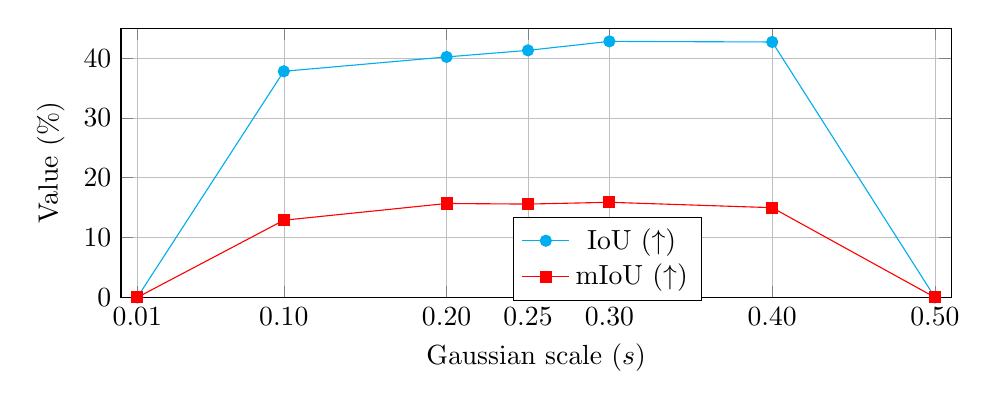
\begin{tikzpicture}
    \begin{axis}[
        width=\columnwidth, %
        height=5cm, %
        xlabel={Gaussian scale ($s$)},
        ylabel={Value (\%)},
        xmin=0, xmax=0.51,
        ymin=0, ymax=45,
        xtick={0.01, 0.10, 0.20, 0.25, 0.30, 0.40, 0.50},
        xticklabels={0.01, 0.10, 0.20, 0.25, 0.30, 0.40, 0.50},
        ytick={0, 10, 20, 30, 40}, %
        legend style={at={(0.7, 0.3)}}, %
        grid=both,
        grid style={line width=.1pt, draw=gray!10},
        major grid style={line width=.2pt, draw=gray!50},
    ]
        \addplot[
            color=cyan,
            mark=*,
            mark options={solid, fill=cyan},
        ] coordinates {
            (0.01, 0.0)
            (0.10, 37.8)
            (0.20, 40.2)
            (0.25, 41.3)
            (0.30, 42.8)
            (0.40, 42.7)
            (0.50, 0.0)
        };
        \addlegendentry{IoU ($\uparrow$)}

        \addplot[
            color=red,
            mark=square*,
            mark options={solid, fill=red},
        ] coordinates {
            (0.01, 0.0)
            (0.10, 12.9)
            (0.20, 15.7)
            (0.25, 15.6)
            (0.30, 15.9)
            (0.40, 15.0)
            (0.50, 0.0)
        };
        \addlegendentry{mIoU ($\uparrow$)}
    \end{axis}
\end{tikzpicture}
    \caption{\textbf{Impact of fixed Gaussian scales on 3D mIoU and IoU} using TPVFormer \cite{huang2023tpv} trained using only $L_{\text{2D}}$ without $L_{\text{3D}}$ on 20\% of Occ3d-nuScenes \cite{tian2023occ3d} validation dataset.}
    \label{fig:impact_of_scale}
\end{figure}


Our results, shown in \autoref{fig:impact_of_scale}, highlight the importance of the Gaussian scale. If the Gaussians are too large, only a few will cover the image, and the loss will be backpropagated mainly from the nearest ones. If they are too small, gaps appear between voxels, leading to sparse activations and a model that renders mostly the empty class, yielding poor metrics.

Theoretically, the optimal size should correlate with the voxel size. For Occ3d-nuScenes and SurroundOcc-nuScenes, the optimal scale is $s = 0.25$ and $s = 0.20$, while for SSCBench-KITTI360, it is $s = 0.1$. This aligns with our intuition: a voxel should be represented by a spherical Gaussian with a standard deviation such that $2s = c$, where $c$ is the voxel side.

Qualitatively, \autoref{fig:impact_of_scale} shows the effect of scale on rendering, confirming the need for a balanced Gaussian size to avoid either sparse activation or excessive concentration on nearby elements.



\begin{figure}[!t]
    \centering
    \begin{subfigure}{0.32\linewidth}
        \includegraphics[width=\linewidth]{fig/scale/occ3d_6e-2.pdf}
        \caption{$\sigma = 0.06$}
    \end{subfigure}
    \hfill
    \begin{subfigure}{0.32\linewidth}
        \includegraphics[width=\linewidth]{fig/scale/occ3d_4e-1.pdf}
        \caption{$\sigma = 0.2$}
    \end{subfigure}
    \hfill
    \begin{subfigure}{0.32\linewidth}
        \includegraphics[width=\linewidth]{fig/scale/occ3d_2e-1.pdf}
        \caption{$\sigma = 0.4$}
    \end{subfigure}

    \vspace{1em} %

    \begin{subfigure}{0.48\linewidth}
        \includegraphics[width=\linewidth]{fig/scale/kitti360_6e-2.pdf}
        \caption{$\sigma = 0.06$}
    \end{subfigure}
    \hfill
    \begin{subfigure}{0.48\linewidth}
        \includegraphics[width=\linewidth]{fig/scale/kitti360_2e-1.pdf}
        \caption{$\sigma = 0.2$}
    \end{subfigure}

    \caption{\textbf{Visualization of different Gaussianized voxels for different datasets and scales}. The first row represents data from Occ3d-nuScenes \cite{tian2023occ3d} and the second and third rows are from SSCBench-Kitti360 \cite{li2024sscbench}.}
    \label{fig:scale_render}
\end{figure}


\subsection{Loss balance}

We {investigate the importance of the balance} $\lambda$ between the 2D loss and the 3D loss. If the {weight of the} 2D loss is too high, there is a risk of optimizing the image rendering at the expense of voxel predictions. Conversely, if the 2D loss is too low, its contribution to the learning process may be {overlooked}. To analyze this, we vary the {contribution $\lambda$ of the 2D loss} and study the impact on the final metrics, {as reported in} \autoref{fig:lambda_impact}. Based on the training results of TPVFormer \cite{huang2023tpv} on a subset of Occ3D-nuScenes \cite{tian2023occ3d}, we set the weight to $\lambda=15$.


\begin{figure}[!t]
    \centering
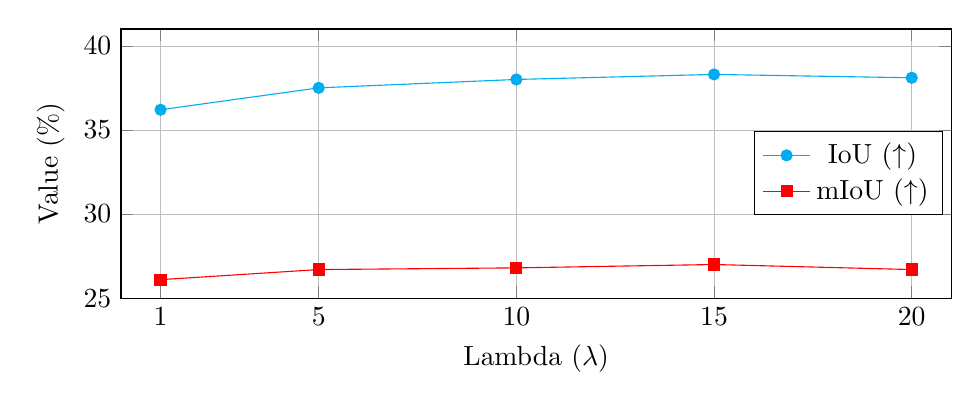
\begin{tikzpicture}
    \begin{axis}[
        width=\columnwidth,
        height=5cm,
        xlabel={Lambda ($\lambda$)},
        ylabel={Value (\%)},
        xmin=0, xmax=21,
        ymin=25, ymax=41,
        xtick={1, 5, 10, 15, 20},
        xticklabels={1, 5, 10, 15, 20},
        ytick={25, 30, 35, 40},
        legend style={at={(0.99, 0.62)}},
        grid=both,
        grid style={line width=.1pt, draw=gray!10},
        major grid style={line width=.2pt, draw=gray!50},
    ]
        \addplot[
            color=cyan,
            mark=* ,
            mark options={solid, fill=cyan},
        ] coordinates {
            (1, 36.2)
            (5, 37.5)
            (10, 38.0)
            (15, 38.3)
            (20, 38.1)
        };
        \addlegendentry{IoU ($\uparrow$)}

        \addplot[
            color=red,
            mark=square*,
            mark options={solid, fill=red},
        ] coordinates {
            (1, 26.1)
            (5, 26.7)
            (10, 26.8)
            (15, 27.0)
            (20, 26.7)
        };
        \addlegendentry{mIoU ($\uparrow$)}
    \end{axis}
\end{tikzpicture}
    \caption{\textbf{Impact of different the contribution $\lambda$ of $L_{2D}$ on 3D semantic occupancy performance.} The architecture used is TPVFormer \cite{huang2023tpv}. Models are trained using a combination of $L_{\text{2D}}$ and $L_{\text{3D}}$ with varying $\lambda$ values and evaluated on 3D IoU and mIoU. We train and evaluate the models on 20\% of Occ3D-nuScenes \cite{tian2023occ3d} training and validation datasets.}
    \label{fig:lambda_impact}
\end{figure}


\subsection{Cameras}
\label{app:ablation:camera}

{
For a given input, we can position as many cameras as needed to render multiple views. In this experiment, we explore using multiple cameras by selecting from the six available views.
While, in theory, more cameras could provide more accurate gradients, we observe in practice that it does not significantly impact the final results (\autoref{fig:num_cams_impact}).
Since additional cameras introduce computational overhead, we opt to render from a single camera per iteration, changing its position across batches according to the strategy defined in \autoref{sec:methods:camera}.
}


\begin{figure}[!t]
    \centering
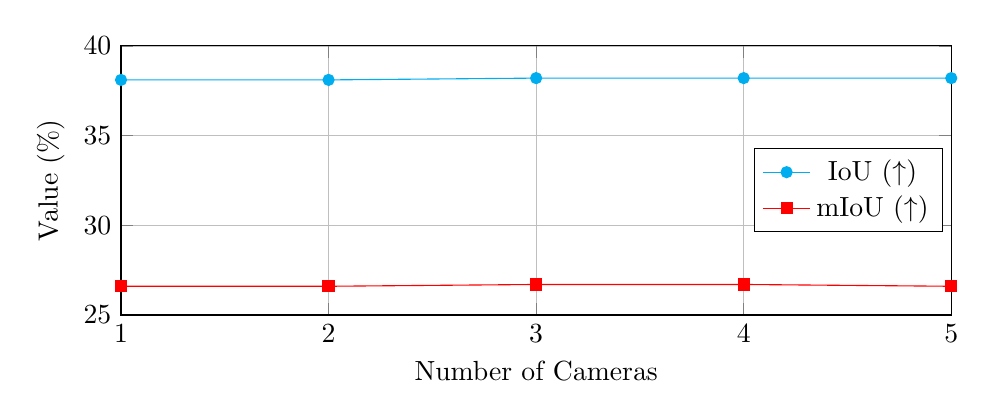
\begin{tikzpicture}
    \begin{axis}[
        width=\columnwidth,
        height=5cm,
        xlabel={Number of Cameras},
        ylabel={Value (\%)},
        xmin=1, xmax=5,
        ymin=25, ymax=40,
        xtick={1, 2, 3, 4, 5},
        xticklabels={1, 2, 3, 4, 5},
        ytick={25,30,35, 40},
        legend style={at={(0.99, 0.62)}},
        grid=both,
        grid style={line width=.1pt, draw=gray!10},
        major grid style={line width=.2pt, draw=gray!50},
    ]
        \addplot[
            color=cyan,
            mark=* ,
            mark options={solid, fill=cyan},
        ] coordinates {
            (1, 38.1)
            (2, 38.1)
            (3, 38.2)
            (4, 38.2)
            (5, 38.2)
        };
        \addlegendentry{IoU ($\uparrow$)}

        \addplot[
            color=red,
            mark=square*,
            mark options={solid, fill=red},
        ] coordinates {
            (1, 26.6)
            (2, 26.6)
            (3, 26.7)
            (4, 26.7)
            (5, 26.6)
        };
        \addlegendentry{mIoU ($\uparrow$)}
    \end{axis}
\end{tikzpicture}
    \caption{\textbf{Impact of the number of cameras on 3D semantic occupancy performance.} The architecture used is TPVFormer \cite{huang2023tpv}. Models are trained with varying numbers of cameras and evaluated on 3D IoU and mIoU using 20\% of Occ3d-nuScenes training and validation set.}
    \label{fig:num_cams_impact}
\end{figure}


\section{Scores detailed per class}
\label{app:results}

The following tables give the detailed IoU and mIoU scores of the models studied for each dataset. \autoref{tab:Occ3d-nuScenes} concerns the Occ3D-nuScenes dataset \cite{tian2023occ3d}, \autoref{tab:SSCBench-KITTI360} the SSCBench-KITTI360 dataset \cite{li2024sscbench} and  \autoref{tab:SurroundOcc-Nuscenes} the SurroundOcc-nuScenes dataset \cite{wei2023surroundocc}. 

\section{Qualitative results}
\label{app:qualitative}
In \autoref{fig:qualitative_0} and \autoref{fig:qualitative_1}, we respectively present qualitative results on randomly selected scenes from SurroundOcc-nuScenes \cite{wei2023surroundocc} and Occ3d-nuScenes datasets \cite{tian2023occ3d}. We also provide complete gifs in our github.


\begin{table*}[t] %
    \small
    \setlength{\tabcolsep}{0.005\linewidth}  
    \centering
    \resizebox{\textwidth}{!}{
    \begin{tabular}{l|c c | c c c c c c c c c c c c c c c c}
        \toprule
        Model
 &  IoU
 &  mIoU
 &  \rotatebox{90}{\textcolor{nbarrier}{$\blacksquare$} barrier}
 &  \rotatebox{90}{\textcolor{nbicycle}{$\blacksquare$} bicycle}
 &  \rotatebox{90}{\textcolor{nbus}{$\blacksquare$} bus}
 &  \rotatebox{90}{\textcolor{ncar}{$\blacksquare$} car}
 &  \rotatebox{90}{\textcolor{nconstruct}{$\blacksquare$} const. veh.}
 &  \rotatebox{90}{\textcolor{nmotor}{$\blacksquare$} motorcycle}
 &  \rotatebox{90}{\textcolor{npedestrian}{$\blacksquare$} pedestrian}
 &  \rotatebox{90}{\textcolor{ntraffic}{$\blacksquare$} traffic cone}
 &  \rotatebox{90}{\textcolor{ntrailer}{$\blacksquare$} trailer}
 &  \rotatebox{90}{\textcolor{ntruck}{$\blacksquare$} truck}
 &  \rotatebox{90}{\textcolor{ndriveable}{$\blacksquare$} drive. suf.}
 &  \rotatebox{90}{\textcolor{nother}{$\blacksquare$} other flat}
 &  \rotatebox{90}{\textcolor{nsidewalk}{$\blacksquare$} sidewalk}
 &  \rotatebox{90}{\textcolor{nterrain}{$\blacksquare$} terrain}
 &  \rotatebox{90}{\textcolor{nmanmade}{$\blacksquare$} manmade}
 &  \rotatebox{90}{\textcolor{nvegetation}{$\blacksquare$} vegetation}
        \\
        \midrule
        MonoScene \cite{cao2022monoscene} & 23.96 & 7.31 & 4.03 &	0.35& 8.00& 8.04&	2.90& 0.28& 1.16&	0.67&	4.01& 4.35&	27.72&	5.20& 15.13&	11.29&	9.03&	14.86 \\
        Atlas \cite{murez2020atlas} & 28.66 & 15.00 & 10.64&	5.68&	19.66& 24.94& 8.90&	8.84&	6.47& 3.28&	10.42&	16.21&	34.86&	15.46&	21.89&	20.95&	11.21&	20.54 \\
        BEVFormer \cite{li2022bevformer} & 30.50 & 16.75 & 14.22 &	6.58 & 23.46 & 28.28& 8.66 &10.77& 6.64& 4.05& 11.20&	17.78 & 37.28 & 18.00 & 22.88 & 22.17 & {13.80} &	{22.21}\\
        TPVFormer-lidar \citep{huang2023tpv} & 11.51 & 11.66 & 16.14&	7.17& 22.63	& 17.13 & 8.83 & 11.39 & 10.46 & 8.23&	9.43 & 17.02 & 8.07 & 13.64 & 13.85 & 10.34 & 4.90 & 7.37\\
        OccFormer \citep{zhang2023occformer} & {31.39} & {19.03} & {18.65} & {10.41} & {23.92} & {30.29} & {10.31} & {14.19} & {13.59} & {10.13} & {12.49} & {20.77} & {38.78} & 19.79 & 24.19 & 22.21 & {13.48} & {21.35}\\
        GaussianFormer \citep{huang2024gaussian} & 29.83 & {19.10} & {19.52} & {11.26} & {26.11} & {29.78} & {10.47} & {13.83} & {12.58} & {8.67} & {12.74} & {21.57} & {39.63} & {23.28} & {24.46} & {22.99} & 9.59 & 19.12 \\
        GaussianFormerv2 \citep{huang2024gaussianformer2} & 30.56 & 20.02 & 20.15 & 12.99 & 27.61 & 30.23 & {11.19} & 15.31 & 12.64 & 9.63 & 13.31 & 22.26 & 39.68 & 23.47 & 25.62 & 23.20 & 12.25 & 20.73 \\ 
        \midrule
        TPVFormer \citep{huang2023tpv} & {30.86} & 17.10 & 15.96&	 5.31& 23.86	& 27.32 & 9.79 & 8.74 & 7.09 & 5.20& 10.97 & 19.22 & {38.87} & {21.25} & {24.26} & {23.15} & 11.73 & 20.81\\
        
        \rowcolor{Apricot!20!}
        \hspace{0.3cm} w/ \method{} & 32.05 & \textbf{20.85} & 20.2 & 13.06 & \textbf{28.95} & 30.96 & \textbf{11.26} & \textbf{16.69} & 13.64 & 10.57 & 12.77 & 22.58 & 40.69 & 23.49 & \textbf{26.41} & 24.97 & 14.41 & 22.94 \\        
        
        (gain) & \textcolor{ForestGreen}{1.19} & \textcolor{ForestGreen}{3.75} & \textcolor{ForestGreen}{4.24} & \textcolor{ForestGreen}{7.75} & \textcolor{ForestGreen}{5.09} & \textcolor{ForestGreen}{3.64} & \textcolor{ForestGreen}{1.47} & \textcolor{ForestGreen}{7.95} & \textcolor{ForestGreen}{6.55} & \textcolor{ForestGreen}{5.37} & \textcolor{ForestGreen}{1.80} & \textcolor{ForestGreen}{3.36} & \textcolor{ForestGreen}{1.82} & \textcolor{ForestGreen}{2.24} & \textcolor{ForestGreen}{2.15} & \textcolor{ForestGreen}{1.82} & \textcolor{ForestGreen}{2.68} & \textcolor{ForestGreen}{2.13} \\ \midrule

        SurroundOcc \cite{wei2023surroundocc} & 31.49 & 20.30 & 20.59 & 11.68 & 28.06 & 30.86 & 10.70 & 15.14 & \textbf{14.09} & \textbf{12.06} & \textbf{14.38} & 22.26 & 37.29 & 23.70 & 24.49 & 22.77 & 14.89 & 21.86 \\
        
        \rowcolor{Apricot!20!}
        \hspace{0.3cm} w/ \method{} & \textbf{32.61} & 20.82 & \textbf{20.32} &\textbf{ 13.22} & 28.32 & \textbf{31.05} & 10.92 & 15.65 & 12.84 & 8.91 & 13.29 & \textbf{22.76} & \textbf{41.22} & \textbf{24.48} & 26.38 & \textbf{25.20} & \textbf{15.31} & \textbf{23.25} \\
        
        (gain) & \textcolor{ForestGreen}{1.12} & \textcolor{ForestGreen}{0.52} & \textcolor{red}{-0.27} & \textcolor{ForestGreen}{1.54} & \textcolor{ForestGreen}{0.26} & \textcolor{ForestGreen}{0.19} & \textcolor{ForestGreen}{0.22} & \textcolor{ForestGreen}{0.51} & \textcolor{red}{-1.25} & \textcolor{red}{-3.15} & \textcolor{red}{-1.09} & \textcolor{ForestGreen}{0.50} & \textcolor{ForestGreen}{3.93} & \textcolor{ForestGreen}{0.78} & \textcolor{ForestGreen}{1.89} & \textcolor{ForestGreen}{2.43} & \textcolor{ForestGreen}{0.42} & \textcolor{ForestGreen}{1.39} \\
        \bottomrule
    \end{tabular}}
    \caption{\textbf{Semantic voxel occupancy results on the \textbf{SurroundOcc-NuScenes} \citep{wei2023surroundocc} validation set.} The best results are in bold. Training models with our module \method{} achieves state-of-the-art performance. Previous results are reported from \cite{huang2024gaussianformer2}.}
    \label{tab:SurroundOcc-Nuscenes}
\end{table*}

\begin{table*}[t] %
    \small
    \setlength{\tabcolsep}{0.005\linewidth}  
    \centering
    \resizebox{\textwidth}{!}{
    \begin{tabular}{l|c|c|c|cccccccccccccccc}
        \hline
        Method & Input & mIoU 
 &  \rotatebox{90}{\textcolor{nother}{$\blacksquare$} others }
 &  \rotatebox{90}{\textcolor{nbarrier}{$\blacksquare$} barrier}
 &  \rotatebox{90}{\textcolor{nbicycle}{$\blacksquare$} bicycle}
 &  \rotatebox{90}{\textcolor{nbus}{$\blacksquare$} bus}
 &  \rotatebox{90}{\textcolor{ncar}{$\blacksquare$} car}
 &  \rotatebox{90}{\textcolor{nconstruct}{$\blacksquare$} const. veh.}
 &  \rotatebox{90}{\textcolor{nmotor}{$\blacksquare$} motorcycle}
 &  \rotatebox{90}{\textcolor{npedestrian}{$\blacksquare$} pedestrian}
 &  \rotatebox{90}{\textcolor{ntraffic}{$\blacksquare$} traffic cone}
 &  \rotatebox{90}{\textcolor{ntrailer}{$\blacksquare$} trailer}
 &  \rotatebox{90}{\textcolor{ntruck}{$\blacksquare$} truck}
 &  \rotatebox{90}{\textcolor{ndriveable}{$\blacksquare$} drive. suf.}
 &  \rotatebox{90}{\textcolor{nother}{$\blacksquare$} other flat}
 &  \rotatebox{90}{\textcolor{nsidewalk}{$\blacksquare$} sidewalk}
 &  \rotatebox{90}{\textcolor{nterrain}{$\blacksquare$} terrain}
 &  \rotatebox{90}{\textcolor{nmanmade}{$\blacksquare$} manmade}
 &  \rotatebox{90}{\textcolor{nvegetation}{$\blacksquare$} vegetation} \\ \hline
        MonoScene & Voxels & 6.06 & 1.75 & 7.23 & 4.26 & 4.93 & 9.38 & 5.67 & 3.98 & 3.01 & 5.90 & 4.45 & 7.17 & 14.91 & 6.32 & 7.92 & 7.43 & 1.01 & 7.65 \\
        BEVDet & Voxels & 19.38 & 4.39 & 30.31 & 0.23 & 32.26 & 34.47 & 12.97 & 10.34 & 10.36 & 6.26 & 8.93 & 23.65 & 52.27 & 24.61 & 26.06 & 22.31 & 15.04 & 15.10 \\
        OccFormer & Voxels  & 21.93 & 5.94& 30.29 & 12.32 & 34.40 & 39.17 & 14.44 & 16.45 & 17.22 & 9.27 & 13.90 & 26.36 & 50.99 & 30.96 & 34.66 & 22.73 & 6.76 & 6.97  \\
        BEVStereo& Voxels & 24.51 & 5.73& 38.41 &7.88 & 38.70 & 41.20 &17.56 &17.33 &14.69 &10.31 &16.84 &29.62 &54.08 &28.92 &32.68 &26.54 &18.74 &17.49 \\ 
        BEVFormer & Voxels & 26.88 & 5.85 & 37.83 & 17.87 & 40.44 & 42.43 & 7.36 & 23.88 & 21.81 & 20.98 & 22.38 & 30.70 & 55.35 & 28.36 & 36.0 & 28.06 & 20.04 & 17.69  \\

        CTF-Occ & Voxels & 28.53 & 8.09 & 39.33 & 20.56 & 38.29 & 42.24 & 16.93 & 24.52 & 22.72 & 21.05 & 22.98 & 31.11 & 53.33 & 33.84 & 37.98 & 33.23 & 20.79 & 18.0 \\
        
        
        RenderOcc & Lidar & 23.93 & 5.69 &27.56 &14.36 &19.91 &20.56 &11.96 &12.42 &12.14 &14.34 &20.81 &18.94 & \textbf{68.85} &33.35 &42.01 &43.94 &17.36 &22.61  \\     
        RenderOcc & Voxels+Lidar & 26.11 & 4.84 & 31.72 & 10.72 & 27.67 & 26.45 & 13.87 & 18.2 & 17.67 & 17.84 & 21.19 & 23.25 & 63.2 & \textbf{36.42} & \textbf{46.21} & \textbf{44.26} & 19.58 & 20.72 \\ \hline
        
        TPVFormer & Voxels & 27.83 & 7.22 & 38.90 & 13.67 & 40.78 & 45.90 & 17.23 & 19.99 & 18.85 & 14.30 & \textbf{26.69} & \textbf{34.17} & 55.65 & 35.47 & 37.55 & 30.70 & 19.40 & 16.78 \\
        \rowcolor{Apricot!20!}
        \hspace{.3cm} w/ GaussRender & Voxels & 30.48 & 9.84 & 42.3 & 24.09 & 41.79 & 46.49 & 18.22 & 25.85 & 25.06 & 22.53 & 22.9 & 33.34 & 58.86 & 33.19 & 36.57 & 31.84 & 23.55 & 21.8 \\
        (gain) & & \textcolor{ForestGreen}{2.65} & \textcolor{ForestGreen}{2.62} & \textcolor{ForestGreen}{3.40} & \textcolor{ForestGreen}{10.42} & \textcolor{ForestGreen}{1.01} & \textcolor{ForestGreen}{0.59} & \textcolor{ForestGreen}{0.99} & \textcolor{ForestGreen}{5.86} & \textcolor{ForestGreen}{6.21} & \textcolor{ForestGreen}{8.23} & \textcolor{red}{-3.79} & \textcolor{red}{-0.83} & \textcolor{ForestGreen}{3.21} & \textcolor{red}{-2.28} & \textcolor{red}{-0.98} & \textcolor{ForestGreen}{1.14} & \textcolor{ForestGreen}{4.15} & \textcolor{ForestGreen}{5.02}
        \\ \hline

        SurroundOcc  & Voxels & 29.21 & 8.64 & 40.12 & 23.36 & 39.89 & 45.23 & 17.99 & 24.91 & 22.66 & 18.11 & 21.64 & 32.5 & 57.6 & 34.1 & 35.68 & 32.54 & 21.27 & 20.27 \\
        \rowcolor{Apricot!20!}
        \hspace{.3cm} w/ GaussRender & Voxels & 30.38 & 8.87 & 40.98 & 23.25 & 43.76 & 46.37 & 19.49 & 25.2 & 23.96 & 19.08 & 25.56 & 33.65 & 58.37 & 33.28 & 36.41 & 33.21 & 22.76 & 22.19 \\
        (gain) &  & \textcolor{ForestGreen}{1.17} & \textcolor{ForestGreen}{0.23} & \textcolor{ForestGreen}{0.86} & \textcolor{red}{-0.11} & \textcolor{ForestGreen}{3.87} & \textcolor{ForestGreen}{1.14} & \textcolor{ForestGreen}{1.50} & \textcolor{ForestGreen}{0.29} & \textcolor{ForestGreen}{1.30} & \textcolor{ForestGreen}{0.97} & \textcolor{ForestGreen}{3.92} & \textcolor{ForestGreen}{1.15} & \textcolor{ForestGreen}{0.77} & \textcolor{red}{-0.82} & \textcolor{ForestGreen}{0.73} & \textcolor{ForestGreen}{0.67} & \textcolor{ForestGreen}{1.49} & \textcolor{ForestGreen}{1.92} \\ \hline
        \end{tabular}
        }
    \caption{\textbf{Semantic voxel occupancy results on the \textbf{Occ3D-nuScenes} \citep{tian2023occ3d} validation set.} The best results are in bold. Training models with our module \method{} achieves state-of-the-art performance. Previous results are reported from \cite{huang2024gaussianformer2, pan2024renderocc}.}
    \label{tab:Occ3d-nuScenes}
\end{table*}

\begin{table*}[t] %
    \small
    \setlength{\tabcolsep}{0.005\linewidth}  
    \centering
    \resizebox{\textwidth}{!}{
    \begin{tabular}{l|cc|cccccccccccccccccccc}
        \toprule
        Method &
        IoU &
        mIoU &
        \rotatebox{90}{\textcolor{ncar}{$\blacksquare$} car} &
        \rotatebox{90}{\textcolor{nbicycle}{$\blacksquare$} bicycle} &
        \rotatebox{90}{\textcolor{nmotor}{$\blacksquare$} motorcycle} & 
        \rotatebox{90}{\textcolor{ntruck}{$\blacksquare$} truck} &
        \rotatebox{90}{\textcolor{nother}{$\blacksquare$} other veh.} &
        \rotatebox{90}{\textcolor{npedestrian}{$\blacksquare$} person} &
        \rotatebox{90}{\textcolor{ndriveable}{$\blacksquare$} road} &
        \rotatebox{90}{\textcolor{nother}{$\blacksquare$} parking} &
        \rotatebox{90}{\textcolor{nsidewalk}{$\blacksquare$} sidewalk} &
        \rotatebox{90}{\textcolor{nother}{$\blacksquare$} other grnd.} &
        \rotatebox{90}{\textcolor{nmanmade}{$\blacksquare$} building} &
        \rotatebox{90}{\textcolor{nmanmade}{$\blacksquare$} fence} &
        \rotatebox{90}{\textcolor{nvegetation}{$\blacksquare$} vegetation} & 
        \rotatebox{90}{\textcolor{nterrain}{$\blacksquare$} terrain} &
        \rotatebox{90}{\textcolor{nmanmade}{$\blacksquare$} pole} &
        \rotatebox{90}{\textcolor{ntraffic}{$\blacksquare$} traf.-sign} &
        \rotatebox{90}{\textcolor{nmanmade}{$\blacksquare$} other struct.} &
        \rotatebox{90}{\textcolor{nother}{$\blacksquare$} other obj.} \\
        \midrule
        MonoScene * & 37.87 & 12.31 & 19.34 & 0.43 & 0.58 & 8.02 & 2.03 & 0.86 & 48.35 & 11.38 & 28.13 & 3.32 & 32.89 & 3.53 & 26.15 & 16.75 & 6.92 & 5.67 & 4.20 & 3.09 \\
        VoxFormer * & 38.76 & 11.91 & 17.84 & 1.16 & 0.89 & 4.56 & 2.06 & 1.63 & 47.01 & 9.67 & 27.21 & 2.89 & 31.18 & 4.97 & 28.99 & 14.69 & 6.51 & 6.92 & 3.79 & 2.43 \\
        OccFormer * & 40.27 & 13.81 & 22.58 & 0.66 & 0.26 & 9.89 & 3.82 & 2.77 & 54.30 & 13.44 & 31.53 & 3.55 & {36.42} & 4.80 & 31.00 & {\textbf{19.51}} & 7.77 & 8.51 & 6.95 & 4.60 \\
        \hline
        SurroundOcc & 38.51 & 13.08 & 21.31 & 0.0 & 0.0 & 6.05 & 4.29 & 0.0 & 53.88 & 12.56 & 30.89 & 2.57 & 34.93 & 3.59 & 29.03 & 16.98 & 5.61 & 6.66 & 4.39 & 2.62 \\
        \rowcolor{Apricot!20!}
        \hspace{.3cm} w/ GaussRender & 38.62 & 13.34 & 21.61 & 0.0 & 0.0 & 6.75 & 4.5 & 0.0 & 53.64 & 11.93 & 30.24 & 2.67 & 35.01 & 4.55 & 29.81 & 17.32 & 6.19 & 8.49 & 4.8 & 2.59 \\
        (gain) & \textcolor{ForestGreen}{0.11} & \textcolor{ForestGreen}{0.26} & \textcolor{ForestGreen}{0.30} & 0.0 & 0.0 & \textcolor{ForestGreen}{0.70} & \textcolor{ForestGreen}{0.21} & 0.0 & \textcolor{red}{-0.24} & \textcolor{red}{-0.63} & \textcolor{red}{-0.65} & \textcolor{ForestGreen}{0.10} & \textcolor{ForestGreen}{0.08} & \textcolor{ForestGreen}{0.96} & \textcolor{ForestGreen}{0.78} & \textcolor{ForestGreen}{0.34} & \textcolor{ForestGreen}{0.58} & \textcolor{ForestGreen}{1.83} & \textcolor{ForestGreen}{0.41} & \textcolor{red}{-0.03} \\  
        \hline 
        Symphonies (official checkpoint) & 43.40 & 17.82 & 26.86 & 4.21 & 4.92 & 14.19 & 7.67 & \textbf{16.79} & 57.31 & 13.60 & 35.25 & 4.58 & 39.20 & \textbf{7.96} & 34.23 & 19.20 & 8.22 & \textbf{16.79} & 6.03 & 6.03 \\
        \rowcolor{Apricot!20!}
        \hspace{.3cm} w/ GaussRender & \textbf{44.08} & \textbf{18.11} & \textbf{27.37} & 3.24 & \textbf{5.12} & \textbf{14.69} & \textbf{8.76} & 16.70 & \textbf{58.05} & \textbf{13.87} & \textbf{35.70} & \textbf{4.76} & \textbf{40.09} & 7.88 & \textbf{34.76} & 19.20 & \textbf{8.22} & 16.49 & \textbf{8.64 }& \textbf{6.50} \\
        (gain) &
        \textcolor{ForestGreen}{+0.68} & \textcolor{ForestGreen}{+0.29} & \textcolor{ForestGreen}{+0.51} & \textcolor{red}{-0.97} & \textcolor{ForestGreen}{+0.20} &
        \textcolor{ForestGreen}{+0.50} & \textcolor{ForestGreen}{+1.09} & \textcolor{red}{-0.09} & \textcolor{ForestGreen}{+0.74} & \textcolor{ForestGreen}{+0.27} &
        \textcolor{ForestGreen}{+0.45} & \textcolor{ForestGreen}{+0.18} & \textcolor{ForestGreen}{+0.89} & \textcolor{red}{-0.08} & \textcolor{ForestGreen}{+0.53} &
        \textcolor{gray}{0.00} & \textcolor{gray}{0.00} & \textcolor{red}{-0.30} & \textcolor{ForestGreen}{+2.61} & \textcolor{ForestGreen}{+0.47} \\
        \bottomrule
    \end{tabular}}
    \caption{\textbf{Semantic voxel occupancy results on the \textbf{SSCBench-KITTI360} \citep{li2024sscbench} test set.} The best results are in bold. Training models with our module \method{} achieves state-of-the-art performance. Previous results are reported from \cite{jiang2024symphonies}.}
    \label{tab:SSCBench-KITTI360}
    \end{table*}



\begin{table*}[ht!]
\centering
\footnotesize
\renewcommand{\arraystretch}{1.2}
\begin{tabular}{p{2.15cm} p{14.05cm}}
\toprule
 & \includegraphics[height=2.6cm]{figure/qualitative_example.pdf}\\
\midrule
Original \phantom{00000} Description & Bromazepam binds to the GABA receptor GABA-A, causing a conformational change and \textbf{increasing inhibitory effects of GABA}. Other neurotransmitters are not influenced. One of the \textbf{benzodiazepines} that is \textbf{used in the treatment of anxiety disorders.} \\
\midrule
User & Explain the features of the given molecule that are most distinct from those of other molecules. \\
\midrule
Mol-LLaMA (Ours) & The given molecule is a member of the \textcolor{tabblue}{benzodiazepine class}, which is characterized by a fusion of a benzene ring and a seven-membered diazepine ring. This structure is crucial for its biological activity, particularly its role as \textcolor{tabblue}{a sedative and hypnotic agent}. ...$<$omitted$>$...\\

& The given molecule is also characterized by a ketone group within the diazepine ring, which is a common feature in benzodiazepines. \textcolor{tabblue}{This functional group is important for the interaction with the GABA-A receptor, enhancing the inhibitory effects of GABA}. ...$<$omitted$>$...\\

\midrule
GPT-4o & 1. **Quinazoline Core**: The molecule contains a \textcolor{tabred}{quinazoline core}, ...$<$omitted$>$... \\
 & Overall, the combination of a \textcolor{tabred}{quinazoline} structure with unique substitution patterns, including bromine halogenation and the presence of a pyridinyl group, ...$<$omitted$>$... . \\
\midrule
LLaMo & The molecule has a \textcolor{tabblue}{benzodiazepine} structure with a bromo substituent at the 7-position and \textcolor{tabred}{a methyl group at the 1-position}. It is distinct from other molecules in that it contains a bromine atom, a nitrogen atom, and a methyl group, which are not present in the other molecules. \\
\midrule
3D-MoLM & ...$<$omitted$>$... It belongs to the class of compounds called \textcolor{tabred}{quinazolines}, which are characterized by a bicyclic structure consisting of a benzene ring fused to a pyrimidine ring. ...$<$omitted$>$...\\
& The molecule's structure suggests potential applications in medicinal chemistry, as quinazolines have been found to possess various biological activities, including \textcolor{tabred}{antitumor, antimicrobial, and anti-inflammatory properties.} \\
\midrule
Mol-Instructions & The molecule is a \textcolor{tabred}{quinoxaline derivative}. \\
\bottomrule
\end{tabular}
\vspace{-0.1in}
\caption{\small Case study to compare molecular understanding and reasoning ability. Mol-LLaMA accurately understands the molecular features, answering a correct molecular taxonomy and providing its distinct properties that are relevant to the given molecule.}
\label{tab:qualitative}
\vspace{-0.1in}
\end{table*}
